\documentclass[acmtog]{acmart}
\usepackage{adjustbox}
\usepackage{subcaption}
\begin{document}

%%
%% The "title" command has an optional parameter,
%% allowing the author to define a "short title" to be used in page headers.
\title{Poster Abstract: Forecasting Renewable Energy at European  Markets
%Time series forecasting of European Energy Market
}

%%
%% The "author" command and its associated commands are used to define
%% the authors and their affiliations.
%% Of note is the shared affiliation of the first two authors, and the
%% "authornote" and "authornotemark" commands
%% used to denote shared contribution to the research.
\author{Hun Rim}
% \authornote{}
\email{rimh@usi.ch}
\author{Juraj Kardos}
\email{juraj.kardos@usi.ch}
\author{Olaf Schenk}
\authornotemark[1]
\email{olaf.schenk@usi.ch}
\affiliation{%
  \institution{Università della Svizzera italiana}
  \streetaddress{Via Giuseppe Buffi 13}
  \city{Lugano}
  \state{Ticino}
  \country{Switzerland}
  \postcode{6900}
}

%%
%% The abstract is a short summary of the work to be presented in the
%% article.
\begin{abstract}
The ambitious energy targets, accelerated by the recent energy crisis, are driving the increase of renewable energy share in gross energy consumption.
% to 42.5\%\cite{eu_renewable_energy}by 2030 from the current 23\%
However, the intermittent and seasonal nature of renewable energy sources presents challenges in predicting their production capacity. The ability to accurately forecast the evolution of renewable energy’s stake in the dynamic and ever-evolving energy market is a critical component in the decision making process of policy makers, and market participants alike. This project aims to explore and evaluate the performance of well-established forecasting methods in anticipating the trends of individual renewable energy components, ultimately contributing to the fostering of a balanced, sustainable, and reliable energy market in the EU. 
%
The primary focus is to assess auto-regressive forecasting methods and advanced models incorporating moving-average, exploit seasonality of time series data, or those utilising the correlation with exogenous variables. The results are presented for data considering recent history of the most significant enegy component at the European energy markets.
%Furthermore, To get a better understanding of not only accuracy, but precision of the models, short-term forecasts are made iteratively to provide a bigger pool of model performance samples. All model’s performance in forecasting the individual energy components are evaluated by measuring and visualising the  Root Mean Square Percentage Error between forecast result and the test data. \\

\end{abstract}

\keywords{Data analytics, Forecasting for energy systems, Energy Market, Renewable energy}
\maketitle

\section{Introduction}
Policymakers and other energy market participants often stress that they need the grid operational statistics faster \cite{eu_nowcasting}, particularly the European energy supply including renewable energy components, and consumption. The goal of the project is to develop a framework for forecasting the individual energy components contributing to the overall energy balance. The framework consists of well-established forecasting methods which can be easily applied to the energy market data, compare the forecast of various methods and asses the their reliability.

%Like a staple good, we have steady demand for energy in our daily lives unlike luxury goods. When visualized, monthly energy demand reveals distinct patterns, with cyclical peaks occurring during winter and lows in summer, notably in July and August. These observations highlight Europe's heightened energy consumption in colder seasons and highlight the data's \textbf{seasonality}, suggesting the possibility of translating these patterns into mathematical models for forecasting future values.\\ 

\subsection{ARIMA}
ARIMA model is one of the most widely used statistical forecasting model \cite{enders2014introduction}. It is a generalized version of AutoRegressive Moving-Average (ARMA) model and difference between the two models is their ability to handle non-stationary data. %Stationarity indicates constancy of statistical property of a dataset such as variance, or mean over time. When data is stationary, it guarantees the stability of underlying patterns in the dataset, and eradicates the concern of the pattern being a result of random fluctuation. ARIMA model is capable of adjusting the data to provide this stability unlike ARMA. \\
Autoregression is a technique used in time series analysis that assumes temporal trend between the values in the dataset, and uncover a function of order \textit{p}. In the auto-regression model, the variable regresses against itself. 
%Put simply, the current value is calculated using past values, by estimating the influence of these past values on the present value. However, even if we assume the general trend is captured perfectly, there are inconsistent white-noise in the data which are not replicable. 
ARIMA model \cite{hong2019core} improves the accuracy by factoring in the non-stationarity of the data. All these factors are combined to formularize ARIMA model as the following:

\begin{equation}
    \hat{L}_N^{(d)} = C + \sum_{i=1}^{p} \psi_i L_{N - i}^{(d)} + \sum_{j=1}^{q}\varphi_j\epsilon_{N-j} + \epsilon_{N}
\end{equation}

\subsection{SARIMA \& SARIMAX}
EU energy market data often exhibit seasonal patterns. SARIMA is an extension that considers these seasonal patterns:

\begin{equation}
    SARIMA = \hat{L}_N^{(d)} + \sum_{i=1}^{P}\Phi_i L_{N - im}^{D} + \sum_{j=1}^{Q}\Theta_j \epsilon_{N - jm}  
\end{equation} 

The EU power sector, just like any other sector, experiences volatility due to exogenous factors such as the climate or the economy. The exogenous variable which has influence on the power sector is collected as additional indicators in the SARIMAX model. 

\subsection{Deep-Learning}
Along with predictive statistics, deep learning (DL) is frequently used in forecasting. Especially, DL using Recurrent-Neural-Network (RNN) with Long Short-term Memory (LSTM) layers is very popular with time series forecasting \cite{raval2018forecasting}. RNN repeats the process of aggregation and activation unlike normal neural networks, and LSTM extends the memory of RNNs. This regression like property of RNN makes it very effective when building a forecasting model, and it would be interesting to evaluate it's performance in comparison to conventional statistical methods.

\section{Experimental Setup}
This sections presents the setup of the forecasting methods considering in the study and presents the data that will be used to evaluate the forecasting accuracy.

\subsection{Parametrization of the Methods}

%\subsection{Parametrization of the Methods}
The autoregressive models need to be parametrized by a set of parameters ${(p, d, q)}$. Their values are determined by \textit{auto\_arima()}\cite{smith2020automated} function of Python, a built-in grid search algorithm from \textit{pmdarima} library.
To train and measure the performance of the forecasting model, we split our data into two parts, training set and test set. We train the model using 60\% of our data and assign the remaining 40\% as test data set to compare it with the forecast.

For training of the model, Python's functions from ${statsmodels}$ library\cite{raschka2019hands} are used. The calculated order and seasonal order are passed to the trainer functions along with the train data set. Each model has respective trainer function provided from the ${statsmodels}$ library (${ARIMA(), SARIMAX()}$)\cite{medium_time_series_forecasting} and are configured accordingly with required training data, order of auto-regression, differencing, and moving-average. Finally, the model is fitted to the passed training data. 
The trained model is used to make a forecast using the model class's ${Predict()}$\cite{medium_time_series_forecasting} function from the starting month to the ending month, in our case considering an interval of 3 months.
The forecast relies on historical values for estimation, which limits the model's ability to capture incoming trends, resulting in decrease of accuracy as the forecast window increases. To avoid this issue, forecasts are made at quarterly intervals. This approach is particularly necessary because the ARIMA model cannot incorporate new forecast errors into its formula, creating a need for iterative recalculation when the training set is updated. Therefore, we adopt the rolling horizon approach, where after each forecast, the training dataset is expanded by one month, and the model is re-trained before forecasting the future values of subsequent three months. By implementing the rolling horizon approach, the model becomes capable of incorporating real-time updates, mimics continuous learning, and avoids forecasting biases.

\subsection{ Analysis}

The performance of forecasting method is measured in terms of the relative error between predicted and actual values using Root-Mean-Squared-Percentage-Error (RMSPE)\cite{botchkarev_performance_2019}. Lower values in RMSPE indicate better performance. RMSPE measures the average percentage deviation between predicted and actual values, providing a standardized measure of prediction accuracy that is independent of the scale of the data. The data used for forecasting is not normalized and individual energy components have radically different scale. Hence, the RMSPE value provides better insight in evaluating forecasting models.
% \begin{equation}
% \text{RMSPE} = \sqrt{\frac{1}{n} \sum_{i=1}^{n} \left( \frac{(Y_i - \hat{Y}_i)}{Y_i} \right)^2} \times 100
% \end{equation}

\subsection{Data}

The dataset consists of monthly energy components contributing to the energy balance on the supply and demand side. The data are published by the national authorities of European countries (usually the transmission system operators or the national statistical offices) and are collected on the level of the high-voltage transmission grid. The focus of this study is put on the key energy components or the components with the high level of variability, particularly electricity demand, and renewable energy generation such as wind, PV or hydro generation.  Electricity demand  is crucial for understanding how much power the system needs to meet consumer needs. Demand can vary significantly based on seasonal factors (heating/cooling), economic activity, and population growth. The increasing penetration of renewables significantly impacts supply dynamics. Understanding the variability of wind and solar generation, as well as the dispatchability (controllable generation) of hydro, is critical for managing grid integration challenges and optimizing renewable energy utilization. Data from the January of 2016 onwards is chosen as this period coincides with a significant ramp-up of renewable energy deployment across Europe. 

\section{Result \& Discussion}

In this section, the performance of the forecasting models are evaluated through assessing solar energy production forecast in France. 

Table ~\ref{fig:forecast_result} presents the performance of the models in forecasting the solar energy production in France. Each model iteratively forecasts 3 months starting at each month within the historical data ranging from April-September 2023. The RMSPE between the test data and model's forecast is recorded.
\begin{table}
    \centering
    \caption{RMSPE of solar energy quarterly forecast in France}
    \label{fig:forecast_result}
    \resizebox{0.37\textwidth}{!}{
    \begin{tabular}{cccccc}
    \toprule
\textbf{Date} & \textbf{Mean} & \textbf{SARIMA} & \textbf{ARIMA} & \textbf{DL} & \textbf{SARIMAX}\\
\midrule
2023-04-01 & 2501.90 & 11.52 & 10.35 & 5.31 & 5.17 \\
\hline
2023-05-01 & 2668.51 & 9.18 & 8.78 & 11.96 & 5.04 \\
\hline
2023-06-01 & 2667.33 & 5.12 & 7.97 & 4.93 & 4.20 \\
\hline
2023-07-01 & 2523.00 & 5.18 & 8.15 & 7.79 & 3.20 \\
\hline
2023-08-01 & 2161.00 & 8.89 & 8.11 & 14.82 & 3.13 \\
\hline
2023-09-01 & 1574.33 & 19.80 & 8.74 & 11.45 & 4.46 \\
    \bottomrule
    \textit{mean} & & 9.94 & 8.68 & 9.38 & 4.20 \\
    \end{tabular}}
\end{table}
Figure ~\ref{fig:solar_performance_forecast} represents the box-plot of the data from table ~\ref{fig:forecast_result}. This visualization is particularly useful when we are viewing larger scale of performance data from different energy sources and different countries. The visualization of the data highlights accuracy, spread, and anomalies of model's performance. Forecast performance of the models showcased in figure ~\ref{fig:solar_performance_forecast} and table ~\ref{fig:forecast_result} highlights that, in general, SARIMAX model forecasting with collection of hourly data as an exogenous variable is the most accurate with all RMSPE being 3 to 5\% with the median being approximately 4\%. ARIMA model has second lowest median of RMSPE with the highest precision, while SARIMA has lower median but lower precision in comparison to the DL model.

\begin{figure}[htp!]
    \centering
    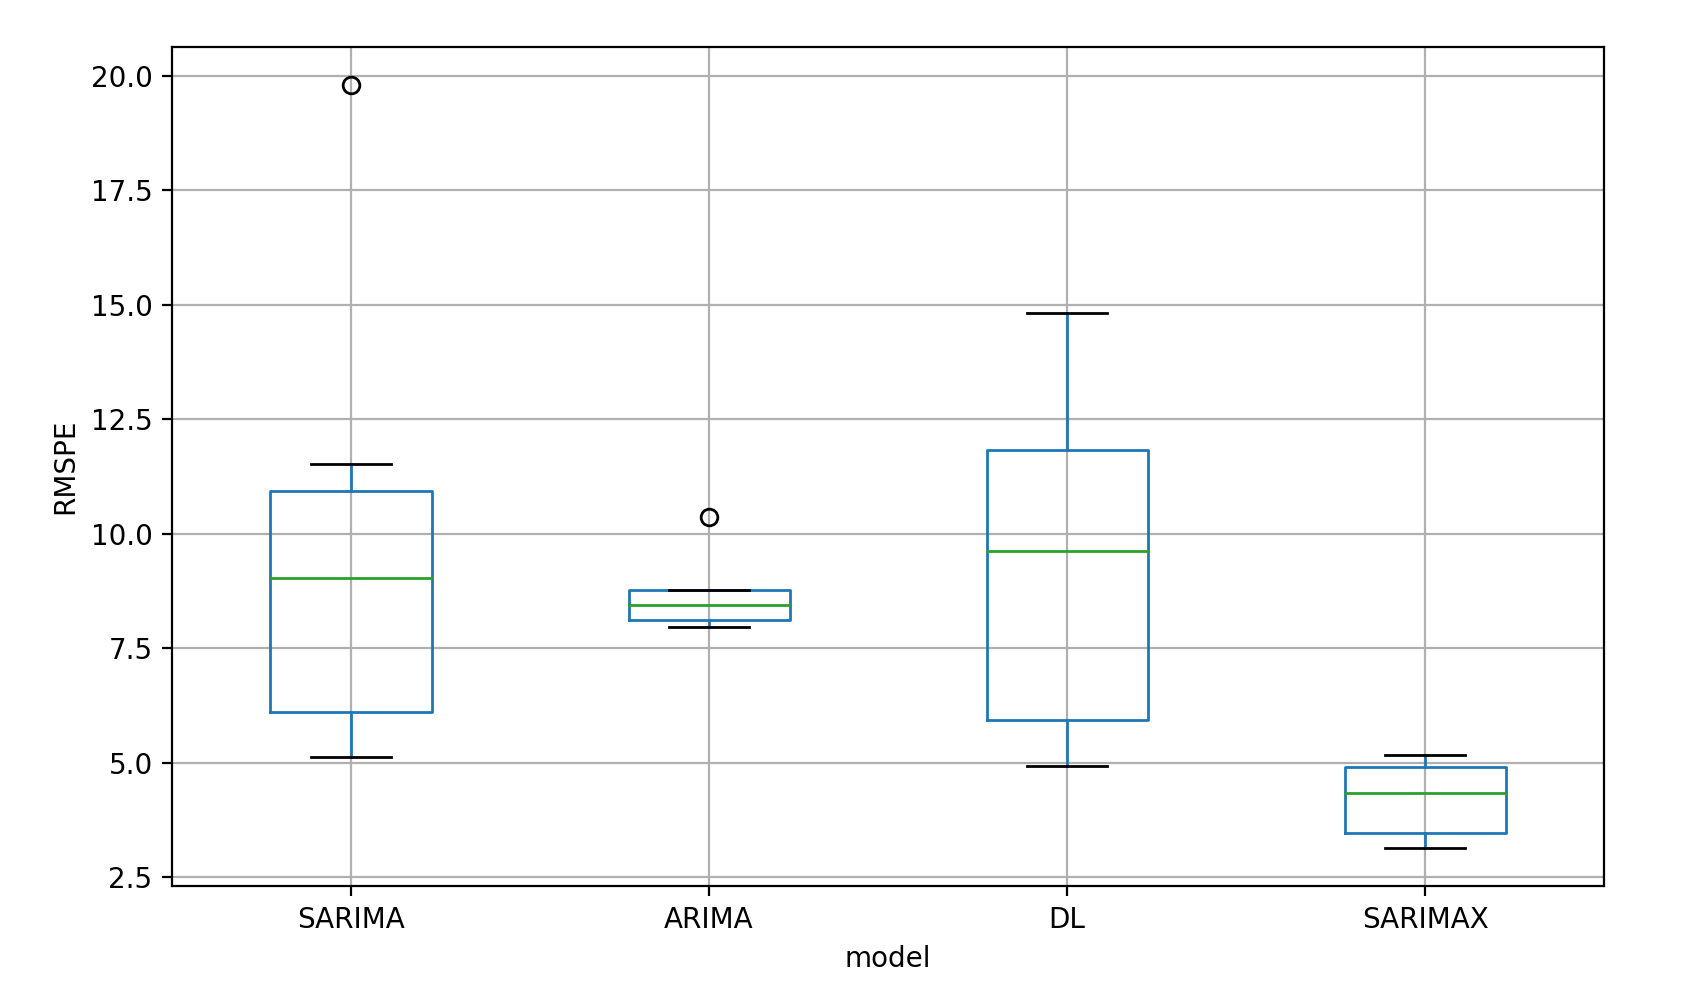
\includegraphics[width=0.42\textwidth, height=4cm]{figures/Figure_3.png}
    \caption{France solar energy production forecast performance visualization}
    \label{fig:solar_performance_forecast} % Tag for referencing
\end{figure}
\begin{figure}[htp!]
    \centering
    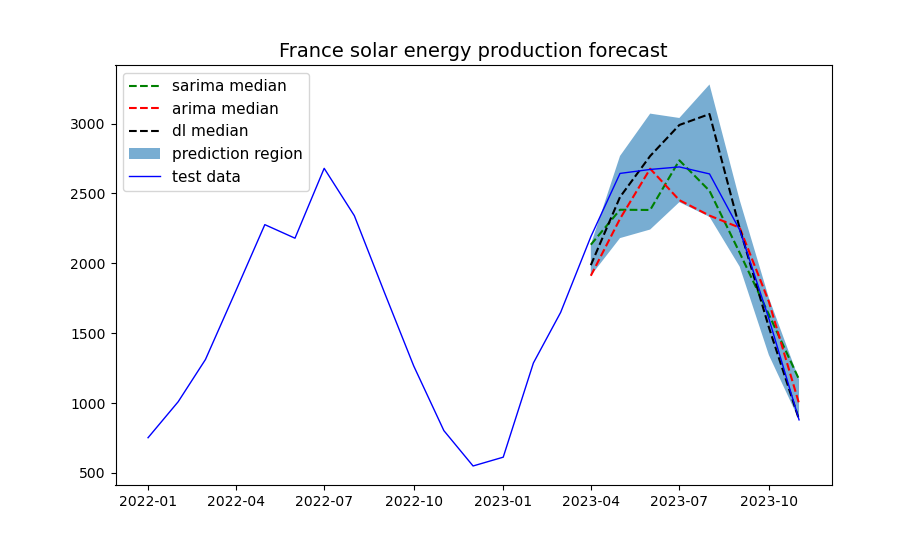
\includegraphics[width=0.42\textwidth]{figures/Figure_1.png}
    \caption{France solar energy production forecast}
    \label{fig:solar_forecast} % Tag for referencing
\end{figure}

Figure ~\ref{fig:solar_forecast} illustrates the median forecast values of each model against the test data, along with a shaded region formed from ensemble of forecasts from all models. The models captured the seasonal trend of declining production from September. However, the solar energy production plateau from May to August was not forecasted by any model. The models tended to predict a peak between June to July as it had occurred in the previous years. Especially the forecast made by the DL model predicted much higher peak and generally higher production of solar energy between May to August (Summer) compared to the true data. This is a reasonable expectation as the computed trend decomposition of solar energy production indicated an ascending trajectory, and in 2023, the production of solar energy surpassed that of previous years for every month until May. Although ARIMA and SARIMA models underestimated the production capacity, their accuracy was higher compared to the DL model. Possible cause for this can be lack of epoches in DL model, or in this case, may be due to sudden increase in residual factors which is visible from seasonal decomposition of the data. Residual factors are accounted for by only statistical models through their MA component. Due to seasonal component, forecasts made by SARIMA in June and July are much more accurate than ARIMA, which already started forecasting a decline in production from May. Forecast from the SARIMAX model is visibly the closest to the test data. Especially, it performs significantly better than SARIMA, its close variant. From this, we can deduce exogenous variables give significant edge to SARIMAX model, and notice the strength of well-chosen exogenous variable. However, while hourly data collection is a great exogenous variable, the time lag between availability of collection of hourly data and monthly data is very short. Hence, SARIMAX model's forecast range gets limited to the lag of the availability. As a result of combining all traits, the ensemble of forecasts accurately delineates the range within which the test data is expected to fall, as depicted by the blue highlighted region in the graph.

% \begin{figure}[htb!]
%     \centering
%     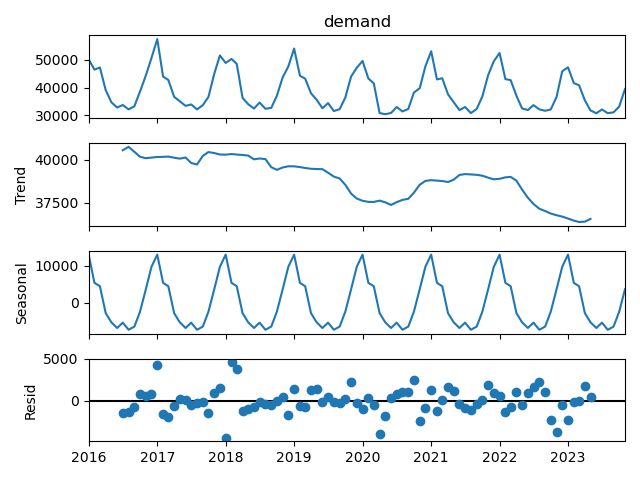
\includegraphics[width=0.49\textwidth]{figures/Figure_4.png}
%     \caption{Seasonal decomposition of solar energy production in France}
%     \label{fig:seasonal_decompose} % Tag for referencing
% \end{figure}

\subsection{Discussion}

As it can be seen in figure ~\ref{fig:3sub1}, ~\ref{fig:3sub2}, and ~\ref{fig:solar_forecast}, complexity of the model does not translate directly to its quality. Almost none of the models perfectly capture the dynamic movement of renewable energy production. Even the SARIMAX model, which has the potential to produce highly accurate and precise forecasts, is constrained by the availability of reliable exogenous variables, which are generally only available for a limited range. However, all models forecast the production capacity to certain accuracy. As it can be seen from the analysis, all models have unique characteristic which makes them perform exceptionally in certain scenarios. While the well-established models are quite accurate on their own, by merging multiple of the well-established models with unique strong suits, it is possible to create a better model. As a simple example, the forecast results of all models are merged to derive a range where the future value may be and it became significantly more reliable. We believe, by choosing right combination of models, it would be possible to create a hybrid model with higher accuracy and precision.

\begin{figure}[htbp]
    \centering
    \begin{subfigure}{0.3\textwidth}
        \centering
        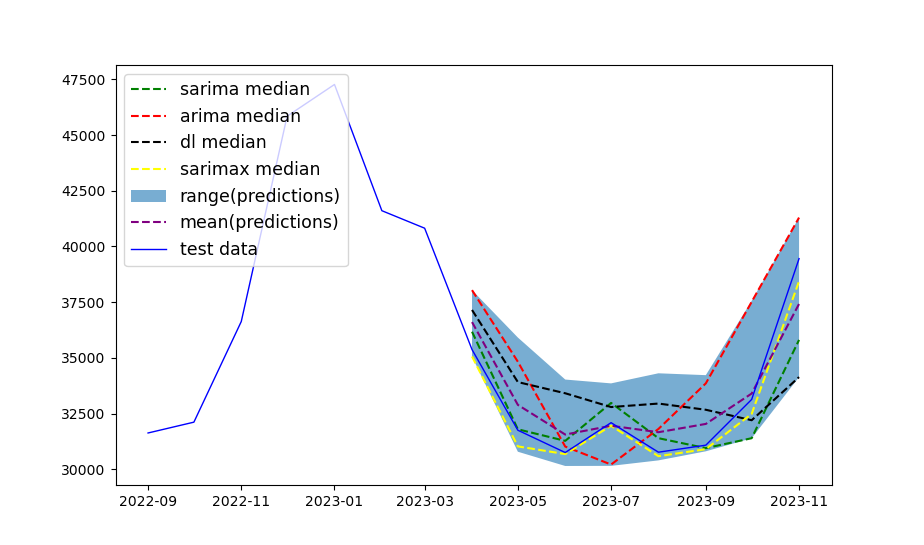
\includegraphics[width=\textwidth]{figures/Figure_5.png}
        \caption{France energy demand forecast}
        \label{fig:3sub1}
    \end{subfigure}
    \hfill
    \begin{subfigure}{0.3\textwidth}
        \centering
        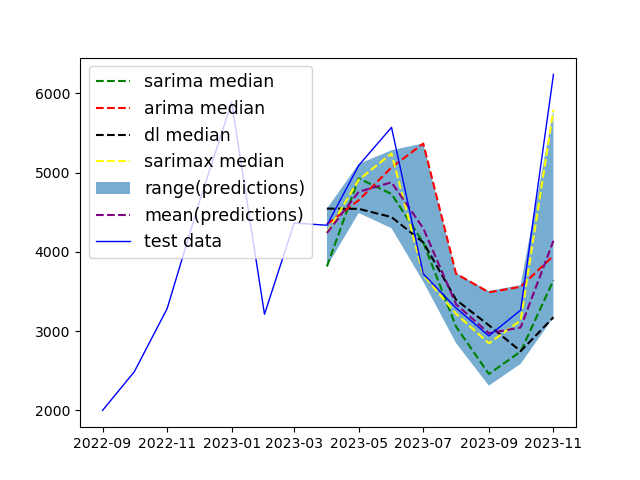
\includegraphics[width=\textwidth]{figures/Figure_6.png}
        \caption{France hydro energy production forecast}
        \label{fig:3sub2}
    \end{subfigure}
    \label{fig:demand_hydro_forecast}
\end{figure}

\section{Conclusion}

This paper has conducted an investigation into the forecasting performance of well-known statistical, and DL methods, providing insights into their strengths and limitations in forecasting demand and production capacity of renewable energies. Through thorough analysis, we have evaluated the effectiveness of these traditional forecasting approaches in evolving European energy market. Our findings demonstrate that while conventional methods such as ARIMA, SARIMA, SARIMAX, and DL models have shown promise in modeling and forecasting renewable energy production, they may have drawbacks or encounter challenges in accurately capturing rapidly shifting trend, seasonality, and residual factors of evolving renewable energy sources. Hence, depending on the properties of the energy components, certain models outperform the others. These challenges underscore the need for tailor-made forecasting methodologies that can better adapt to the complex dynamics of renewable energy production with traditional models as the base. Moving forward, future focus should be on exploring alternative forecasting techniques, such as hybrid models, that better incorporate factors such as weather or economic indicators, technological advancements, and policy changes. By exploiting diverse forecasting methodologies and utilising the advancements in data science, we can enhance the accuracy and reliability of renewable energy production forecasts, thus facilitating the transition towards a sustainable and resilient energy future in Europe.


\bibliographystyle{ACM-Reference-Format}
\bibliography{poster_abstract}


\end{document}

